\documentclass{article}

%packages
\usepackage[margin=1in,a4paper]{geometry}
\usepackage[utf8]{inputenc}
\usepackage[cyr]{aeguill}
\usepackage[french]{babel}
\usepackage{hyperref}
\usepackage{amsmath}
\usepackage{gensymb}
\usepackage{enumitem,amssymb}
\newlist{checks}{itemize}{2}
\setlist[checks]{label=$\square$}
\usepackage{graphicx}
\usepackage{subcaption}
\usepackage{wrapfig}
\usepackage{amsthm}
\usepackage{amsfonts}
\usepackage{pdfpages}
\usepackage{pgfplots}
\pgfplotsset{compat=newest}
\usetikzlibrary{calc}
\usepackage{mathtools}
\usepackage{array}
\usepackage[T1]{fontenc}
\usepackage{lmodern}
\usepackage{tabularx}
\usepackage{fancyhdr}
\usepackage{pst-func}
\usepackage{xcolor}
\usepackage{nicefrac}
\usepackage{mdframed}
\usepackage[boxed,vlined]{algorithm2e}
\usepackage{cleveref}
\newcommand{\Lim}[1]{\raisebox{0.5ex}{\scalebox{1}{$\displaystyle \lim_{#1}\;$}}}
\usepackage{tkz-tab}

\usetikzlibrary{babel}
\usepackage{babel}
\usepackage[european, straightvoltages]{circuitikz}
\usepackage{multicol}

%macros
\newcommand{\R}{\mathbb{R}}
\newcommand{\C}{\mathbb{C}}
\newcommand{\w}{\omega}
\newcommand{\p}{\partial}
\newcommand{\cross}{\times}
\newcommand{\inc}{\fontfamily{cmr}\selectfont\textperiodcentered}
\DeclareMathOperator{\sinc}{sinc}
\DeclareMathOperator{\interior}{int}
\DeclareMathOperator{\adh}{adh}
\DeclareMathOperator{\argcosh}{argcosh}
\DeclareMathOperator{\argsinh}{argsinh}
\DeclareMathOperator{\Ima}{Im}
\usepackage{mathtools, stmaryrd}
\usepackage{xparse} \DeclarePairedDelimiterX{\Iintv}[1]{\llbracket}{\rrbracket}{\iintvargs{#1}}
\NewDocumentCommand{\iintvargs}{>{\SplitArgument{1}{,}}m}
{\iintvargsaux#1} %
\NewDocumentCommand{\iintvargsaux}{mm} {#1\mkern1.5mu..\mkern1.5mu#2}

\title{Introduction à l'électricité}
\author{\href{https://s4s.fun}{\textcolor{blue}{\underline{STUDENTS FOR STUDENTS}}}\\Première édition}
\date{Septembre 2021}

\addto\captionsfrench {
  \renewcommand{\contentsname}%
    {Exercices}%
}

\begin{document}

\pagenumbering{gobble}
\maketitle

\begin{center}
   
\includegraphics[scale=0.5]{Images/ic_launcher.png} 
\end{center}
\vfill
\tableofcontents
\vfill
\newpage

\pagenumbering{arabic}
\setlength{\parskip}{1ex}

\section*{Préambule}

Ces exercices ne ressemblent, pour la plupart, absolument pas aux séries d'exercices que vous aurez pendant l'année. Nous avons fait l'hypothèse qu'il était préférable de tester vos connaissances sur l'introduction à l'électricité que vous venez de suivre, plutôt que de vous balancer une copie des exos que vous aurez de toute manière en grande quantité au cours d'électricité.

De plus, une partie de ces exercices sont assez difficiles, et ne vous découragez donc pas si vous ne voyez pas la solution immédiatement. Réfléchissez un moment, et si vous ne voyez vraiment pas, appelez à l'aide un\inc{}e assistant\inc{}e. Nous vous conseillons également de ne pas passer trop de temps sur chaque exercice, une fois que vous avez trouvé comment faire. Il est préférable d'avoir vu chaque exercice pendant la séance pour poser vos questions aux assistant\inc{}e\inc{}s, quitte à finir les exercices précédents plus tard.

Cela dit, ne vous mettez pas la pression. Comme toutes les séries d'exercices, elle sera probablement trop longue pour être finie pendant la séance. 

\section{Principes physiques et loi d'Ohm}

\subsection{Oiseaux cuits}
\textit{En supposant un courant continu dans le câble}, pourquoi les oiseaux perchés sur des lignes à haute tension ne se font-ils pas électrocuter ? Indiquez le lien avec l'illustration du chat mangeant les charges vue en cours.
\begin{center}
   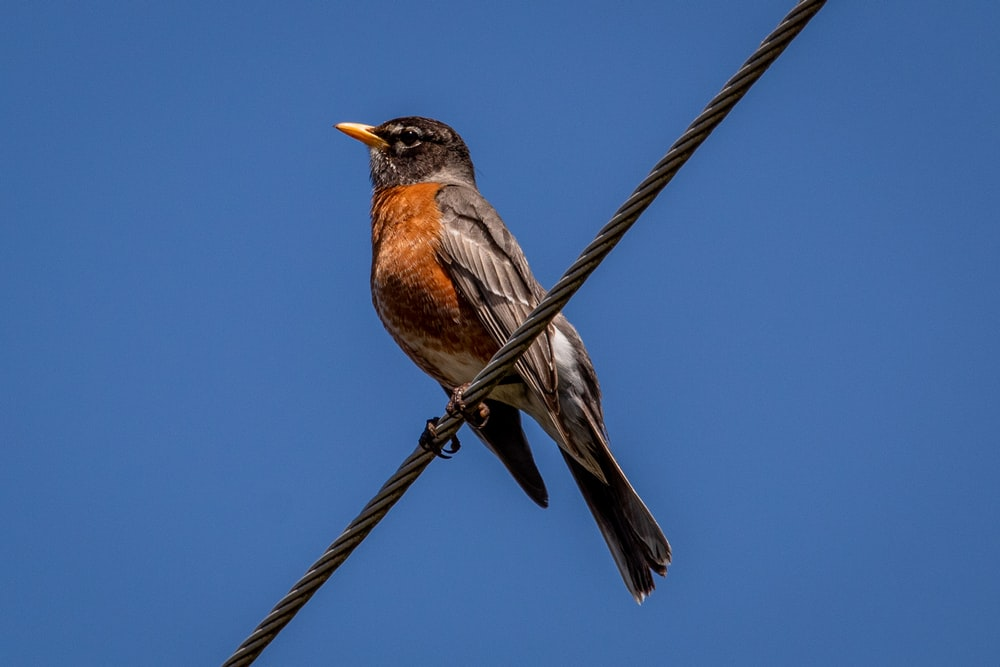
\includegraphics[scale=0.18]{Images/oiseausurfil.png} 
\end{center}

\subsection{pH = 15}
\noindent On va voir les applications les plus basiques de la loi d'Ohm :
\begin{enumerate}
    \item Dans le circuit de gauche, quel courant passe par la résistance avec $U=10 V$ et $R=250 \Omega$?
    \item Quelle résistance serait nécessaire pour obtenir un courant de $0.1 A$ avec $U=15 V$?
    \item Dans le circuit de droite, quelle est la tension aux bornes de la résistance avec $I=0.2 A$ et $R=30 \Omega$?
    \item Quelle résistance serait nécessaire pour obtenir une tension de $20 V$ avec $I=0.4 A$?
\end{enumerate}
\begin{center}
    \begin{tabular}{ccc}
    \begin{circuitikz}
    \draw (0,0) to [V<=$U$] (0,3) to (2,3) to [R, l_=$R$, i>_=$I$](2,0) to [short](0,0);
    \end{circuitikz}
    &
    \hspace{1.5cm}
    &
    \begin{circuitikz}
    \draw (0,0) to [I=$I$] (0,3) to (2,3) to [R, l_=$R$, v^=$U$](2,0) to [short](0,0);
    \end{circuitikz}
\end{tabular}
\end{center}

\subsection{Accidents}
Voici de subtils conseils pour facilement tuer quelqu'un; la résistance du corps est mesurée entre les deux mains, et le graphe n'est utile que pour un courant avec une fréquence de l'ordre des $\SI{50}{Hz}$ habituels:
\begin{center}
    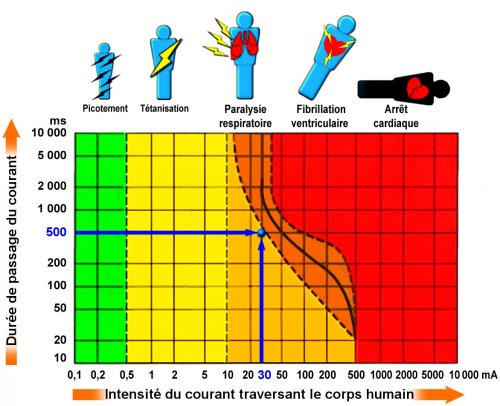
\includegraphics[scale=0.6]{Images/courantduree.jpg}
    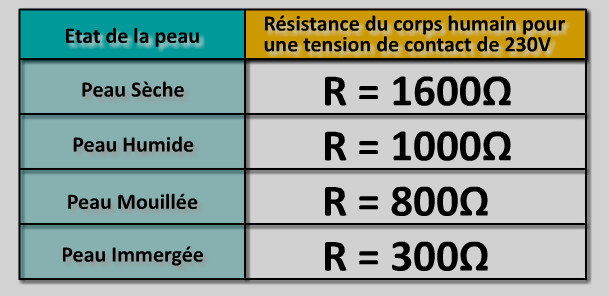
\includegraphics[scale=0.3]{Images/resistancecorps.jpg}
\end{center}
\begin{enumerate}
    \item Calculez les courants pour 230 V dans le corps humain sec, mouillé et immergé pour éventuellement optimiser votre meurtre. Combien de temps faudra-t-il rester exposer dans chaque cas pour que le meurtre aboutisse ?
    \item Une décharge électrostatique à lieu avec une tension d'au moins 3000 V ; pourquoi n'est-elle pas mortelle?
    \item Que pensez vous de la phrase \og Ce n'est pas la tension qui tue, mais le courant \fg ? Selon vous, comment s'applique-t-elle (ou pas) aux décharges électrostatiques ?
\end{enumerate}

\textit{Attention !} Nous avons fait beaucoup de simplification. En pratique, la mortalité de l'électrocution est beaucoup plus compliquée à estimer. Ne pensez surtout pas que cet exercice vous a donné les compétences pour aller toucher les prises de $\SI{230}{\volt}$ sans danger de mort.

\subsection{Ampoule}
Une ampoule à incandescence contient un fil en métal, généralement en tungstène ayant une température de fusion au-delà de 3400°C, par lequel passe une puissance électrique qui est dissipée en chaleur et en lumière par la résistance du fil (celui-ci ne brûle ou s'évapore pas car il est entouré de vide ou d'un gaz non réactif). Pour l'intérêt de cet exercice, on considérera que la luminosité émise est proportionelle à la puissance dissipée.
\begin{enumerate}
    \item Si l'on branche une telle ampoule aux bornes d'une source de courant, est il donc préférable d'utiliser un fil à haute ou faible résistance pour obtenir une luminosité maximale?
    \item Qu'en est-il si l'ampoule est branchée sur une source de tension?
\end{enumerate}
Voici le symbole électrique d'une lampe. Il ne vous aidera pas pour l'exercice, où nous considérons l'ampoule uniquement par sa résistance.
\begin{center}
    \begin{circuitikz}
    \draw (0,0) to [lamp](4,0);
    \end{circuitikz}
\end{center}

\section{Traitement des circuits}

\subsection{A e s t h e t i c s}
\label{exo:aesthetics}

\subsubsection{Un circuit moche}
\label{sexo:circuit_moche}

Simplifiez et clarifiez le circuit suivant en minimisant le nombre de noeuds et en dégageant les branches en parallèle.
\begin{center}
\begin{circuitikz}
\draw
 (0,0) to [european voltage source] (2,0)
 to [R, l^=$R_3$](2,3)
 to [short](2,3.6) 
 to [R, l_=$R_2$](0,3) 
 to [R, l_=$R_1$](0,0) 
 (2,3.4) to [short, *-](3,3.4)
 to [R, l_=$R_5$](5,3.4)
 to [R, l^=$R_6$](5,0.4)
 to[european voltage source, -*](3,0.4)
 (2,2.7) to [short, *-](3.2,2.6)
 to [R, l^=$R_4$](3,0.2)
 to [short, -*](2,0.2)
 (3,3.4) to [short, *-](3,4)
 to [short](6,3.8)
 to [R, l^=$R_7$](6,1)
 to [short, -*](5,0.6)
 ;
\end{circuitikz}
\end{center}

\subsubsection{Résistance équivalente série}    
On cherche des méthodes qui simplifieraient le circuit davantage, et donc un moyen de remplacer plusieurs résistances par une seule, en gardant le même courant et la même chute en tension sur leur branche.

On cherche pour l'instant à remplacer deux résistances $R_1$ et $R_2$ montées en série par une seule résistance équivalente $R_{eq}$, telle que le courant $I$ à travers la branche reste le même pour une même chute de tension $U$:
\begin{center}
\begin{tabular}{m{0.3\textwidth}cm{0.28\textwidth}}
\raggedright
\begin{circuitikz}
\draw
(0,0) to [R, o-, l_=$R_1$, v^=$U_{R_1}$](2,0)
to (2.4, 0)
to [R, l_=$R_2$] (3.6,0)
to [short, i_=$I$, -o] (4.5,0)
(2,0.34) to [open, v^=$U_{R_2}$] (4,0.34)
(0,1) to [open, v^>= $U$](4,1)
;
\end{circuitikz}
&
\centering
\Large $\equiv$
\normalsize
&
\raggedleft
\begin{circuitikz}
\draw
  (0,0) to [short, o-](1,0)
  to [R, l_=$R_{eq}$, v^=$U$] (3,0)
  to [short, i_=$I$, -o](4,0);
\end{circuitikz}
\end{tabular}
\end{center}
Exprimez $R_{eq}$ en fonction de $R_1$ et $R_2$. Indice: exprimez $U$ à gauche avec la loi des mailles, puis la tension à travers $R_1$, $R_2$ et $R_{eq}$ avec la loi d'Ohm.

\subsubsection{Résistance équivalente parallèle}

On cherche maintenant à remplacer deux résistances $R_1$ et $R_2$ montées en parallèle par une seule résistance équivalente $R_{eq}$, telle que la chute de tension $U$ entre les deux bouts reste la même pour un même courant $I$:
\begin{center}
\begin{tabular}{m{0.3\textwidth}cm{0.28\textwidth}}
\raggedright
\begin{circuitikz}
\draw
(0.5,0) to [short, o-*](1,0)
to [short](1,1)
to (1.4,1)
to [R, l_=$R_1$](2.6,1)
to [short, i_=$I_{R_1}$](3.5,1)
to [short](3.5,0)
(1,0) to [short](1,-1)
to (1.4,-1)
to [R, l_=$R_2$](2.6,-1)
to [short, i_=$I_{R_2}$](3.5, -1)
to [short, -*](3.5,0)
to [short, i_=$I$, -o](4.5,0)
(0,1.5) to [open, v^>= $U$](4.5,1.5)
;
\end{circuitikz}
&
\centering
\Large $\equiv$
\normalsize
&
\raggedleft
\begin{circuitikz}
\draw
  (0,0) to [short, o-](1,0)
  to [R, l_=$R_{eq}$, v^=$U$] (3,0)
  to [short, i_=$I$, -o](4,0);
\end{circuitikz}
\end{tabular}
\end{center}
Exprimez $R_{eq}$ en fonction de $R_1$ et $R_2$. Indice: exprimez $I$ à gauche avec la loi des n\oe{u}ds, puis le courant à travers $R_1$, $R_2$ et $R_{eq}$ avec la loi d'Ohm.

\subsubsection{Un circuit joli}

Appliquez les deux dernières méthodes sur le circuit simplifié de l'exercice \ref{sexo:circuit_moche} en combinant les résistances et indiquant la valeur des résistances équivalentes obtenues.

Ces méthodes de simplification de résistances en série et en parallèle seront importantes pour la suite de l'année, et on retrouve des formules analogues pour les capacités et inductances.

\subsection{Diviseur de tension}
Ce type de circuit s'appelle un pont diviseur de tension. Vous le rencontrerez à de nombreuses reprises durant votre première année à l'EPFL et dans toutes les matières électroniques à suivre.
\begin{center}
\begin{circuitikz}[straight voltages]
\draw
  (0,0) to [V<=$U$] (0,3) 
  to [R, l_=$R_1$, v^=$U_{R_1}$] (3,3)
  to [R, l_=$R_2$, v^=$U_{R_2}$] (3,0) 
  to [short, i_=$I$] (0,0);
\end{circuitikz}
\end{center}
\begin{enumerate}
    \item Si vous y arrivez, estimez (sans calculer) comment se comparent $U_{R_1}$ et $U_{R_2}$  en fonction de $R_1$ et $R_2$ (dans les cas $R_1=R_2$, $R_1<R_2$ et $R_1>R_2$).
    \item En appliquant la loi des mailles sur ce circuit, calculez la valeur de $I$ en fonction de $U$, $R_1$ et $R_2$, puis en déduire l'équation de $U_{R_2}$.
    \item Application numérique: Que valent $I$ et $U_{R_2}$ pour $U$ = 5 V, $R_1$ = 5 k$\Omega$ et $R_1$ = 15 k$\Omega$?
\end{enumerate}

%\subsection{Identification de n\oe{}uds, branches et mailles}
%exemples de circuits où il faut trouver noeuds, branches et mailles
% un peu inutile après les exos précédents non?

\subsection{Lois de Kirchhoff}
Dans ce circuit déjà vu en cours, donnez les valeurs des courants $I$, $I_1$ et $I_2$, et des tensions $U_{R_1}$ et $U_{R_2}$, en fonction de $U$, $R_1$, $R_2$ et $R_3$.
\begin{center}
\begin{circuitikz}
\draw
  (0,0) to [V<=$U$] (0,4)
  to [short, i^=$I$] (3,4)
  to [R, l_=$R_3$, i>^=$I_1$] (3,0) 
  to [short, *- ] (0,0)
  (3,4) to [short, *- , i^=$I_2$] (6,4)
  to [R, l_=$R_1$, v^=$U_{R_1}$] (6,2)
  to [R, l_=$R_2$, v^=$U_{R_2}$] (6,0)
  to [short] (3,0);
\end{circuitikz}
\end{center}

\noindent On vous propose la méthode suivante :
\begin{enumerate}
    \item Identifier les n\oe{}uds, les branches, et si vous voulez les mailles.
    \item Énoncer la loi des n\oe{}uds et la loi des mailles (la variante que vous voulez, mais là c'est vraiment plus simple avec la deuxième variante) pour chacun des n\oe{}uds, branches ou mailles que vous avez trouvés. 
    \item Résoudre le système d'équations ainsi obtenu (on peut le résoudre systématiquement de la même manière que vous avez vu en algèbre linéaire, ou le faire plus intuitivement).
\end{enumerate}

\subsection{Lois de Kirchhoff, exemple un peu plus affreux}

Même consigne qu'à l'exo précédent. Exprimez $I_{R_2}$, $I_{R_4}$, $I_{R_8}$, $I_{R_{10}}$, $U_{R_3}$, $U_{R_6}$ et $U_{R_7}$ en fonction de $(R_k)_{1\leq k \leq 10}$, de $U_1$ et de $U_2$.

\begin{enumerate}
    \item Comme c'est un exo sur Kirchhoff, et qu'on aime bien vous embêter, on vous suggère de n'utiliser que les lois d'Ohm et Kirchhoff, et de ne pas utiliser les résultats précédents permettant de simplifier les résistances en série et en parallèle.
    \item  Dans un second temps, recalculez ces valeurs en utilisant les simplifications des résistances équivalentes en série et en parallèle que vous avez calculées dans l'exercice \ref{exo:aesthetics}.
\end{enumerate}

\begin{center}
\begin{circuitikz}
\draw
(0,0) to [R=$R_5$] (0,2)
to [R=$R_3$, v<=$U_{R_3}$] (0,4)
to [R=$R_1$] (0,6)
to [short, -*] (2,6)
to [R=$R_2$] (2,4)
to [short, -*, i=$I_{R_2}$] (0,4)
(0,2) to [R=$R_4$, *-] (2.5,2)
to [short, -*, i=$I_{R_4}$] (2.5,0)
(2,6) to (4,6)
to [V=$U_1$] (4,3)
to [R=$R_6$, v=$U_{R_6}$] (6.5,3)
to [R=$R_{10}$, i>^=$I_{R_{10}}$] (6.5,0)
to [V=$U_2$] (2.5,0)
to (0,0)
(6.5,3) to [R=$R_8$, i<=$I_{R_8}$] (6.5,6)
to [R=$R_7$, v=$U_{R_7}$] (9,6)
to (9,3)
to [R=$R_9$, -*] (6.5,3);
\end{circuitikz}
\end{center}

\subsection{Autre exemple un peu pété}

Donnez tous les courants indiqués et les tensions aux bornes de chaque résistance en fonction de $U$ et de la valeur de chaque résistance. Les flèches des courants sur les schémas ont été dessinées dans un sens arbitraire : vous pouvez donc trouver des résultats négatifs.

\begin{center}
\begin{circuitikz}
\draw
  (0,0) to [R, l_=$R_1$, i^=$i_1$](3,0)
  to [R, *- , l_=$R_2$](6,0)
  to [short](6,-3)
  to [short, i^=$i_2$](3,0)
  to [R, l_=$R_3$, i^=$i_3$](3,-3)
  to [R, *- , l_=$R_4$, i^=$i_4$](0,-6)
  to [R, *- , l_=$R_5$, i^=$i_5$](0,0)
  (0,-6) to [V, v_=$U$](6,-6)
  to [short, i^=$i_6$](3,-3);
\end{circuitikz}
\end{center}

\subsection{Une ampoule sur une pile}

\noindent On branche une ampoule ayant une résistance de $\SI{3}{\ohm}$ sur une pile de $\SI{9}{\volt}$. 

\begin{enumerate}
    \item Représentez la situation sur un schéma électrique. Rappelez-vous qu'une pile est une source de tension réelle.
    \item On constate que l'ampoule dégage une puissance de $\SI{3}{\watt}$.\footnote{On néglige le fait qu'une partie de cette puissance est dissipée sous forme de chaleur et l'autre partie sous forme de lumière. La valeur qu'on vous donne est la puissance totale consommée par l'ampoule.} Quelle est la résistance interne de la pile ?
    \item Quels seraient la tension aux bornes de l'ampoule, le courant la traversant et la puissance qu'elle dissipe, si l'ampoule avait en fait une résistance de $\SI{6}{\ohm}$ ?
    \item Combien de courant traverserait la pile si on la court-circuitait ?
\end{enumerate}

\section{Condensateurs et bobines}

\subsection{Moteur électrique}

Un moteur électrique synchrone fonctionne en faisant passer du courant dans une bobine dans la partie fixe du moteur (le stator), ce qui induit un champ magnétique appliquant une force sur un aimant dans la partie qui tourne (le rotor). 

Cette bobine possède une inductance, et on peut donc représenter le moteur branché à une source par ce schéma très simplifié :

\begin{center}
\begin{circuitikz}
\draw
    (0,0) coordinate (zero) to [V<=$U$] ++(0, 3)
    to [cute opening switch] ++(2.5, 0) coordinate (a)
    to [L, l_=$L$, a^=moteur] (a |- zero)
    to (zero);
\end{circuitikz}
\end{center}

Le trait épais représente un interrupteur, que l'on peut ouvrir pour couper le circuit. Expliquez pourquoi il peut être très dangereux d'ouvrir le circuit quand le moteur est en marche. En pratique, les moteurs possèdent des circuits permettant d'éviter ce problème.

\textit{NB} : en réalité, les moteurs électriques sont alimentés par du courant alternatif, et cela change certaines choses, comme le fait que le courant restera borné. Si vous ne savez pas encore ce qu'est le courant alternatif, vous le verrez en long et en large pendant l'année.

\subsection{Choisissez mieux vos ami\inc{}e\inc{}s}

Votre amie aimerait qu'à chaque fois que vous appuyiez sur un interrupteur, son ampoule s'allume pendant une seconde. Comme vous avez bien suivi le cours, vous pensez à un condensateur. Nous vous proposons le circuit suivant :

\begin{center}
\begin{circuitikz}
\draw
    (0,0) node[cute spdt up arrow, xscale=-1](Sw){}
    (Sw.out 1) to ++(-2.5,0)
    to [V=$\SI{230}{\volt}$] ++(0,-4) coordinate (zero) {} -| (Sw.out 2)
    (Sw.in) to [C=$C$] ++(2.5,0) coordinate (a)
    to [lamp, i>^=$i$, v_=$u$, l=$\SI{880}{\ohm}$] (a |- zero)%c'est le cancer cette notation oh it worked
    to [short, -*] (Sw.out 2 |- zero); %beeeeeh
\end{circuitikz}
\end{center}

\subsubsection{Que va-t-il se passer ?}

Le trait épais relié aux trois ronds représente l'interrupteur, qui peut être dans deux états. Tracez qualitativement les graphes du courant $i$ traversant l'ampoule et de la tension $u$ à ses bornes, en fonction du temps, quand :
\begin{enumerate}
    \item le circuit est resté longtemps avec l'interrupteur vers le haut, et on appuie sur l'interrupteur (on pivote le trait vers le bas).
    \item le circuit est resté longtemps avec l'interrupteur vers le bas, et on appuie sur l'interrupteur (on pivote le trait du bas vers le haut).
\end{enumerate}

Indiquez sur le graphe la valeur du courant et de la tension à l'instant où l'interrupteur change de position, et après avoir attendu longtemps (quand $t \to \infty$).

\subsubsection{Application numérique}

Les courants et tensions dans la dernière question seront des formes
\[
\arraycolsep=20pt
\begin{array}{cc}
    \displaystyle
    K \mathrm{e}^\frac{-t}{RC} & K\left(1-\mathrm{e}^\frac{-t}{RC}\right)
\end{array}\]
où $R$ est la résistance de l'ampoule et $C$ la capacité du condensateur.

\begin{enumerate}
    \item Trouver laquelle des deux formes correspond à chacun des quatre graphes, ainsi que les valeurs de $K$ correspondant.
    \item Trouver la valeur de $C$ de sorte que l'ampoule mette une seconde pour pour perdre $95\%$ du courant qui la traverse, à partir du moment où l'on a appuyé sur l'interrupteur.%Pour corr, ça devrait être 378 uF
\end{enumerate}

\textit{NB} : si vous essayez ce circuit sur le réseau électrique de votre maison (c'est une façon de parler, n'essayez surtout pas !), vous verrez qu'il ne marche pas. En réalité, le courant des prises murales est alternatif, et cela change notamment que le condensateur ne va jamais se charger et arrêter de laisser passer le courant. Le circuit serait donc totalement inefficace.

\subsection{Detective Current}

Simplifiez le circuit suivants et donnez les formules de toutes les tensions (sur chaque n\oe{}ud) et de toutes les intensités de courant (sur chaque branche), en fonction de $U$ et des valeurs des résistances. Le petit symbole en-bas du circuit indique le point du $\SI{0}{\volt}$. Cela veut dire que lorsqu'on vous demande la tension sur un n\oe{}ud, on vous demande en réalité la tension \textit{entre} ce n\oe{}ud et le petit symbole.

On va faire ici une analyse dite \textit{DC} (pour \textit{direct current}), c'est-à-dire qu'on va considérer qu'on a laissé le circuit tranquille pendant très longtemps, et que les bobines et condensateurs sont entièrement chargés, et que respectivement leur courant et leur tension ne changent plus.

\begin{center}
\begin{circuitikz}
\draw
  (0,0) to [R, l_=$R_1$, i^=$i_2$](3,0)
  to [R, l_=$R_2$](5,0)
  to [R, *- , l_=$R_3$, i^=$i_3$](7,0)
  to [R, *-,l_=$R_5$](10,0)
  to [short, i^=$i_5$](10,-5)
  to [short](7,-5)
  (7,0) to [V, v_=$U$, i^=$i_4$](7,-3)
  to [R, l_=$R_4$](7,-5)
  to [short, *- ](5,-5)
  (5,0) to [R, l_=$R_6$, i^=$i_6$](5,-3)
  to [C, l_=$C$](5,-5)
  to [short, *- ](3,-5)
  to [L, l_=$L_2$](0,-5)
  to [R, *- , l_=$R_7$, i^=$i_7$](0,0)
  to [short, *- ](-2,0)
  to [L, l_=$L_1$, i^=$i_1$](-2,-5)
  to [short] (0,-5)
  (4,-5) to [short, *-] (4, -5.5) node[tlground]{};
\end{circuitikz}
\end{center}

\subsection{The secret for always staying down-to-earth}
On arrondit violemment et admet que la masse d'un corps humain est due à $65\%$ à oxygène ${}_8^{16}O$, $20\%$ au carbone ${}_6^{12}C$, $10\%$ à l'hydrogène ${}_1^1H$ et $5\%$ à l'azote ${}_7^{14}N$. Cours de chimie rapide: le nombre en haut est la masse molaire de l'atome, celui en bas son nombre atomique et la constante d'Avogadro est $N_A\approx \SI{6e23}{\per\mole}$.
\begin{enumerate}
    \item Trouvez le nombre d'électrons dans un corps humain de $\SI{65}{\kilogram}$ parce qu'on se marre. D'ailleurs, il faudra amener sa calculatrice à l'exam.
    \item On admet que le corps forme un condensateur d'environ $\SI{100}{\pico\farad}$ avec la Terre, et on rappelle $e = \SI{1.6e-19}{\coulomb}$. Quelle tension y aurait-il entre un être humain et la Terre s'il y avait un 1\% plus d'électrons que de protons dans cet être humain?
    \item Montrer comment un raisonnement similaire explique-t-il pourquoi il est impossible de faire passer un courant dans un circuit ouvert. Avant ça, demandez un joint à Jonas c gratui.
\end{enumerate}

\subsection{Capacité équivalente série}

On aimerait trouver un condensateur de valeur $C_{eq}$ qui se comporte de la même façon que l'ensemble des deux condensateurs de valeur $C_1$ et $C_2$ en série.

\begin{center}
\begin{tabular}{m{0.4\textwidth}cm{0.3\textwidth}}
\centering
\begin{circuitikz}
\draw
    (0,0) to [C=$C_1$, o-] ++(2.5,0)
    to [C=$C_2$, -o] ++(2.5,0);
\end{circuitikz}
&
\centering \Large $\equiv$ \normalsize
&
\centering
\begin{circuitikz}
\draw (0,0) to [C=$C_{eq}$, o-o] (2.5,0);
\end{circuitikz}
\end{tabular}
\end{center}

Indice : considérez le circuit suivant, et utilisez la loi des mailles, la loi des n\oe{}uds et l'équation $Q=Cu$. Cherchez la valeur de $U_1$, $U_2$ et de $Q$ pour chacun des condensateurs.

\begin{center}
\begin{circuitikz}
\draw
    (0,0) to [V<=$U$] ++(0,4)
    to ++(3,0)
    to [C=$C_1$, v=$U_1$] ++(0, -2)
    to [C=$C_2$, v=$U_2$] ++(0, -2)
    to (0,0);
\end{circuitikz}
\end{center}

\subsection{Circuit LC}

Trouvez une analogie hydraulique qui vous permettra de comprendre \emph{qualitativement} (sans faire aucun calcul) ce qui se passera dans ce circuit si l'on part d'une situation où le condensateur est chargé et où la bobine est complètement \og déchargée \fg{}.

\begin{center}
\begin{circuitikz}
\draw
    (0,0) coordinate (zero) to [L=$L$] (0,4)
    to [short, , i=$i(t)$] ++(3, 0) coordinate (a)
    to [C=$C$] (a |- zero)
    to (zero)
    (1.5,4) to [open, v=$u(t)$] ++(0,-4);
\end{circuitikz}
\end{center}

Tracez un graphe approximatif du courant et de la tension (pas besoin d'indiquer l'échelle, ça dépendra évidemment des valeurs $C$ et $L$).

%\subsection{Pour les plus courageux}

%On aimerait vous introduire au courant alternatif et aux impédances des condensateurs et des bobines.

\end{document}